\documentclass[10pt,xcolor={dvipsnames},fleqn]{beamer}
%\documentclass[handout,10pt,xcolor={dvipsnames},fleqn]{beamer}
\usepackage{isse}


\usepackage{apalike}
\usepackage[utf8]{inputenc}
\usepackage{pdfpages}
%\usepackage{ngerman}
\usepackage{stmaryrd,amsmath,amssymb}
\usepackage{color}
\usepackage{enumerate}
\usepackage[makeroom]{cancel}
\usepackage{mdframed}
\usepackage{xskak}
\usepackage{marvosym}
\setchessboard{
showmover=false}
\usepackage[noend]{algpseudocode}   % package for algorithms
\usepackage{algorithm}
\usepackage{tikz}

\usepackage[absolute,overlay]{textpos}

\usetikzlibrary{trees,calc,shapes,arrows,matrix,shadows,decorations.markings}

\mdfdefinestyle{theoremstyle}{
linecolor=red,linewidth=2pt,
frametitlerule=true,
frametitlebackgroundcolor=gray!20,
innertopmargin=\topskip,
}
\definecolor{LRed}{rgb}{1,.8,.8}
\definecolor{MRed}{rgb}{1,.6,.6}
\definecolor{HRed}{rgb}{1,.2,.2}

\usepackage{listings}
\lstdefinelanguage{mzn}
{
	morekeywords={var,int,solve,bool,not,search,satisfy,endif,maximize,minimize,float,constraint,sum,forall,exists,array,of,include,predicate,then,commit,post,set,function,if,else,repeat,next,ann,break},
	sensitive=false,
	morecomment=[l]{\%},
	morecomment=[s]{/*}{*/},
	morestring=[b]",
}

\definecolor{lightlightgray}{gray}{0.95}
\definecolor{forestgreen}{HTML}{009B55}
\definecolor{thermicred}{rgb}{0.82, 0.1, 0.26}
\lstset
{
	basicstyle=\ttfamily\small,
	commentstyle=\ttfamily\color{thermicred},
	stringstyle=\ttfamily\color{isseorange},
	keywordstyle=\ttfamily\color{blue},
	tabsize=2,
	showstringspaces=false,
	flexiblecolumns=true,
	captionpos=b,	
	backgroundcolor=\color{lightlightgray},
	frame=single,
	 xleftmargin=\parindent,
}

\lstset{language=mzn}
\interfootnotelinepenalty=10000

% ====== custom commands

\newcommand{\prosumer}[1]{\ensuremath{\mathtt{#1}}}
% Soft Constraint Example
\newcommand{\constraintName}[1]{\ensuremath{\mathtt{#1}}}
% Biogas Constraints
\newcommand{\biogas}{biogas}
\newcommand{\biogasShort}{bio}
\newcommand{\gasFull}{\ensuremath{\constraintName{gasFull}_\mathtt{\biogasShort}}}
\newcommand{\ecoSweet}{\ensuremath{\constraintName{ecoSweet}_\mathtt{\biogasShort}}}
\newcommand{\onOff}{\ensuremath{\constraintName{onOff}_\mathtt{\biogasShort}}}
% Thermal Plant Constraints
\newcommand{\thermal}{thermal}
\newcommand{\thermalShort}{therm}
\newcommand{\ecoOpt}{\ensuremath{\constraintName{ecoOpt}_\mathtt{\thermalShort}}}
\newcommand{\inertia}{\ensuremath{\constraintName{inertia}_\mathtt{\thermalShort}}}
\newcommand{\ecoGood}{\ensuremath{\constraintName{ecoGood}_\mathtt{\thermalShort}}}
\newcommand{\hLevelThermal}[1]{$H_#1^\mathtt{\thermalShort}$}
% Electric Vehicle
\newcommand{\ev}{EV}
\newcommand{\limitBatteryUsage}{\ensuremath{\constraintName{limitBU}_\mathtt{\ev}}}
\newcommand{\prefBatteryLevel}{\ensuremath{\constraintName{prefBL}_\mathtt{\ev}}}
\newcommand{\earlyBird}{\ensuremath{\constraintName{earlyBird}_\mathtt{\ev}}}
% Organization
\newcommand{\org}{org}
\newcommand{\minMaxViolation}{\ensuremath{\constraintName{violation}_\mathtt{\org}}}
\newcommand{\hLevelOrg}[1]{$H_#1^\mathtt{\org}$}

\newcommand{\Variable}{X}
\newcommand{\LocalVariable}{\widehat{\Variable}}
\newcommand{\Domain}{D}
\newcommand{\Constraint}{C}
\newcommand{\ConstraintRelationship}{\mathcal{R}}

\newcommand{\valuation}{v}
\newcommand{\constraint}[1]{\mathrm{#1}}

\newcommand{\plantconstraint}[3]{  
\ifx#1b \constraint{best}[#3]
\else \ifx#1g \constraint{good}[#3]
\else \ifx#1a \constraint{acc}[#3]
\else \ifx#1d \constraint{diff}
\else \ifx#1l \constraint{low}[#3]
\else \ifx#1h \constraint{high}[#3]
\else \ifx#1o \constraint{org}[#3]
   \else
   \constraint{#1}_{#2}^{#3} 
   
   
\fi \fi \fi \fi \fi \fi \fi}
\usepackage{stmaryrd}

\providecommand{\smyth}[1]{\prec^{#1}}
\providecommand{\smytheq}[1]{\preceq^{#1}}

\providecommand{\checkfull}{\color{ForestGreen} \checkmark}
\providecommand{\checkhalf}{\color{BurntOrange} (\checkmark)}
\providecommand{\checknot}{\color{BrickRed} $x$}
% booktabs, tables 
\usepackage{booktabs}
\usepackage{tabularx}
\usepackage{longtable}
\usepackage{dcolumn}
\newcolumntype{R}{>{\raggedleft\arraybackslash}X}
\newcolumntype{d}[1]{D{.}{.}{#1} }
\newcolumntype{L}[1]{>{\raggedright\let\newline\\\arraybackslash\hspace{0pt}}m{#1}}


\newcommand{\code}[1]{\normalfont\texttt{\spaceskip=3pt\frenchspacing\def\{{\char123}\def\}{\char125}\def\^{\char94}\def\_{\char95}#1}}
\newcommand{\varit}[1]{{\frenchspacing\ensuremath{\normalfont\textsl{#1}}}}
\newcommand{\macit}[1]{{\frenchspacing\ensuremath{\normalfont\textsf{#1}}}}
\newcommand{\Eta}{\mathrm{H}}
\newcommand{\Mu}{\mathrm{M}}
\newcommand{\Nu}{\mathrm{N}}

\newcommand{\NZ}{\mathbb{N}}
\newcommand{\RZ}{\mathbb{R}}
\newcommand{\RZp}{\RZ_{\geq 0}}
\newcommand{\powerset}{\mathcal{P}}
\newcommand{\limp}{\mathrel{\Rightarrow}}
\newcommand{\compfun}{\mathbin{\circ}}
\newcommand{\isorel}{\mathrel{\cong}}
\newcommand{\restrict}[2]{{#1}\mathnormal{\upharpoonright}{#2}}
\newcommand{\natto}{\mathrel{\dot{\mathnormal{\to}}}}
\let\lbagold\lbag
\let\rbagold\rbag
\def\lbag{\mathopen{\lbagold}}
\def\rbag{\mathclose{\rbagold}}

\DeclareMathOperator{\Minop}{\mathrm{Min}}
\newcommand{\Min}[1]{\Minop^{#1}}
\DeclareMathOperator{\Maxop}{\mathrm{Max}}
\newcommand{\Max}[1]{\Maxop^{#1}}
\DeclareMathOperator{\finsets}{\mathcal{P}_{\mathrm{fin}}}
\DeclareMathOperator{\nefinsets}{\mathcal{P}_{\mathrm{fin}^+}}
%\DeclareMathOperator{\incfinsets}{\mathcal{I}_{\mathrm{fin}}}
\newcommand{\incfinsets}[1]{\mathcal{I}_{\mathrm{fin}}^{#1}}
\newcommand{\lowersubseteq}[1]{\mathrel{\subseteq_{#1}}}
\newcommand{\lowersupseteq}[1]{\mathrel{\supseteq_{#1}}}
\newcommand{\lowersubset}[1]{\mathrel{\subset_{#1}}}
\newcommand{\lowersupset}[1]{\mathrel{\supset_{#1}}}
\newcommand{\uppersubseteq}[1]{\mathrel{\subseteq^{#1}}}
\newcommand{\uppersupseteq}[1]{\mathrel{\supseteq^{#1}}}
\newcommand{\uppersubset}[1]{\mathrel{\subset^{#1}}}
\newcommand{\uppersupset}[1]{\mathrel{\supset^{#1}}}
\newcommand{\lowercup}[1]{\mathbin{\cup_{#1}}}
\newcommand{\uppercup}[1]{\mathbin{\cup^{#1}}}

\DeclareMathOperator{\finmsets}{\mathcal{M}_{\mathrm{fin}}}
\DeclareMathOperator{\nefinmsets}{\mathcal{M}_{\mathrm{fin}^+}}
\newcommand{\mcup}{\mathbin{\mathnormal{\cup}\llap{\text{\fontsize{8pt}{8pt}\selectfont$-$}}}}
\newcommand{\submseteq}{%
\mathrel{\mathchoice%
{\mathnormal{\subseteq}\llap{\text{\raisebox{0.3pt}{\fontsize{8pt}{8pt}\selectfont\rotatebox{90}{$-$}\hspace{1.8pt}}}}}%
{\mathnormal{\subseteq}\llap{\text{\raisebox{0.3pt}{\fontsize{8pt}{8pt}\selectfont\rotatebox{90}{$-$}\hspace{1.8pt}}}}}%
{\mathnormal{\subseteq}\llap{\text{\raisebox{-0.3pt}{\fontsize{5pt}{5pt}\selectfont\rotatebox{90}{$-$}\hspace{1.4pt}}}}}%
{\mathnormal{\subseteq}\llap{\text{\raisebox{-0.3pt}{\fontsize{5pt}{5pt}\selectfont\rotatebox{90}{$-$}\hspace{1.4pt}}}}}%
}}
\newcommand{\supmseteq}{\mathrel{\reflectbox{$\submseteq$}}}
\newcommand{\lowersubmseteq}[1]{\mathrel{\submseteq_{#1}}}
\newcommand{\uppersubmseteq}[1]{\mathrel{\submseteq^{#1}}}
\newcommand{\submset}{%
\mathrel{\mathchoice%
{\mathnormal{\subset}\llap{\text{\raisebox{-0.8pt}{\fontsize{8pt}{8pt}\selectfont\rotatebox{90}{$-$}\hspace{1.8pt}}}}}%
{\mathnormal{\subset}\llap{\text{\raisebox{-0.8pt}{\fontsize{8pt}{8pt}\selectfont\rotatebox{90}{$-$}\hspace{1.8pt}}}}}%
{\mathnormal{\subset}\llap{\text{\raisebox{-0.3pt}{\fontsize{7pt}{7pt}\selectfont\rotatebox{90}{$-$}\hspace{1pt}}}}}%
{\mathnormal{\subset}\llap{\text{\raisebox{-0.3pt}{\fontsize{7pt}{7pt}\selectfont\rotatebox{90}{$-$}\hspace{1pt}}}}}%
}}
\newcommand{\supmset}{\mathrel{\reflectbox{$\submset$}}}
\newcommand{\lowersubmset}[1]{\mathrel{\submset_{#1}}}
\newcommand{\uppersubmset}[1]{\mathrel{\submset^{#1}}}

\DeclareMathOperator{\collapseset}{\mathcal{C}}

\newcommand{\category}[1]{\mathrm{#1}}
\newcommand{\POcat}{\category{PO}}
\newcommand{\uSLcat}{\category{uSL}}
\newcommand{\poMoncat}{\category{poMon}}
\newcommand{\jMoncat}{\category{jMon}}
\newcommand{\mMoncat}{\category{mMon}}
\newcommand{\xMoncat}{{x}\category{Mon}}
\newcommand{\PVScat}{\category{PVS}}
\newcommand{\cSRngcat}{\category{cSRng}}
\newcommand{\DAGcat}{\category{DAG}}

\newcommand{\idfun}[1]{1_{#1}}
\newcommand{\functor}[1]{\mathit{#1}}
\DeclareMathOperator{\POfun}{\functor{PO}}
\DeclareMathOperator{\uSLfun}{\functor{uSL}}
\DeclareMathOperator{\poMonfun}{\functor{poMon}}
\DeclareMathOperator{\jMonfun}{\functor{jMon}}
\DeclareMathOperator{\mMonfun}{\functor{mMon}}
\DeclareMathOperator{\xMonfun}{\text{$x$}\functor{Mon}}
\DeclareMathOperator{\PVSfun}{\functor{PVS}}
\DeclareMathOperator{\cSRngfun}{\functor{cSRng}}
\DeclareMathOperator{\DAGfun}{\functor{DAG}}

\newcommand{\uSLfree}[1]{\uSLfun\langle#1\rangle}
\newcommand{\uSLeta}{\eta^{\uSLcat}}
\newcommand{\uSLetaat}[1]{\uSLeta_{#1}}
\newcommand{\uSLlift}[1]{{#1}^{\sharp_{\uSLcat}}}

\newcommand{\poMonfree}[1]{\poMonfun\langle#1\rangle}
\newcommand{\poMoneta}{\eta^{\poMoncat}}
\newcommand{\poMonetaat}[1]{\poMoneta_{#1}}
\newcommand{\poMonlift}[1]{{#1}^{\sharp_{\poMoncat}}}

\newcommand{\jMonfree}[1]{\jMonfun\langle#1\rangle}
\newcommand{\jMoneta}{\eta^{\jMoncat}}
\newcommand{\jMonetaat}[1]{\jMoneta_{#1}}
\newcommand{\jMonlift}[1]{{#1}^{\sharp_{\jMoncat}}}

\newcommand{\mMonfree}[1]{\mMonfun\langle#1\rangle}
\newcommand{\mMoneta}{\eta^{\mMoncat}}
\newcommand{\mMonetaat}[1]{\mMoneta_{#1}}
\newcommand{\mMonlift}[1]{{#1}^{\sharp_{\mMoncat}}}

\newcommand{\PVSfree}[1]{\PVSfun\langle#1\rangle}
\newcommand{\PVSeta}{\eta^{\PVScat}}
\newcommand{\PVSetaat}[1]{\PVSeta_{#1}}
\newcommand{\PVSlift}[1]{{#1}^{\sharp_{\PVScat}}}

\newcommand{\xMonfree}[1]{\xMonfun\langle#1\rangle}
\newcommand{\xMoneta}{\eta^{\xMoncat}}
\newcommand{\xMonetaat}[1]{\xMoneta_{#1}}
\newcommand{\xMonlift}[1]{{#1}^{\sharp_{\xMoncat}}}

\newcommand{\cSRngfree}[1]{\cSRngfun\langle#1\rangle}
\newcommand{\cSRngeta}{\eta^{\cSRngcat}}
\newcommand{\cSRngetaat}[1]{\cSRngeta_{#1}}
\newcommand{\cSRnglift}[1]{{#1}^{\sharp_{\cSRngcat}}}

\newcommand{\POfree}[1]{\POfun\langle#1\rangle}
\newcommand{\POeta}{\eta^{\POcat}}
\newcommand{\POetaat}[1]{\POeta_{#1}}
\newcommand{\POlift}[1]{{#1}^{\sharp_{\POcat}}}

\newcommand{\mtimes}[1]{\mathbin{\tilde{\cdot}_{#1}}}
\newcommand{\mplus}[1]{\mathbin{\tilde{\cup}_{#1}}}
\newcommand{\ftimes}[1]{\mathbin{\tilde{\mcup}^{#1}}}
\newcommand{\fplus}[1]{\mathbin{\tilde{\cup}_{#1}}}

\DeclareMathOperator{\scope}{\mathrm{sc}}
\DeclareMathOperator{\defdom}{\mathrm{def}}

\newcommand{\reflclos}[1]{\mathrel{(#1)^=}}
\newcommand{\transclos}[2][+]{\mathrel{(#2)^{#1}}}
\newcommand{\refltransclos}[1]{\mathrel{(#1)^*}}

\newcommand{\XPDrel}[2][\pi]{\rightsquigarrow^{#1}_{#2}}
\newcommand{\XPDreleq}[2][\pi]{\rightsquigarrow^{#1, =}_{#2}}
\newcommand{\XPDord}[2][\pi]{<^{#1}_{#2}}
\newcommand{\XPDordeq}[2][\pi]{\geq^{#1}_{#2}}
\newcommand{\XPDleq}[2][\pi]{\leq^{#1}_{#2}}
\newcommand{\XPDgeq}[2][\pi]{\geq^{#1}_{#2}}
\newcommand{\XPDw}[2][\pi]{w^{#1}_{#2}}
\newcommand{\XPDW}[2][\pi]{W^{#1}_{#2}}
\newcommand{\XPDk}[2][\pi]{k^{#1}_{#2}}

\newcommand{\SPDrel}{\XPDrel[\mathrm{SPD}]}
\newcommand{\SPDreleq}{\XPDreleq[\mathrm{SPD}]}
\newcommand{\SPDleq}{\XPDleq[\mathrm{SPD}]}
\newcommand{\SPDgeq}{\XPDgeq[\mathrm{SPD}]}
\newcommand{\SPDord}{\XPDord[\mathrm{SPD}]}
\newcommand{\SPDw}{\XPDw[\mathrm{SPD}]}
\newcommand{\SPDW}{\XPDW[\mathrm{SPD}]}
\newcommand{\DPDrel}{\XPDrel[\mathrm{DPD}]}
\newcommand{\DPDreleq}{\XPDreleq[\mathrm{DPD}]}
\newcommand{\DPDord}{\XPDord[\mathrm{DPD}]}
\newcommand{\DPDw}{\XPDw[\mathrm{DPD}]}
\newcommand{\DPDW}{\XPDW[\mathrm{DPD}]}
\newcommand{\TPDrel}{\XPDrel[\mathrm{TPD}]}
\newcommand{\TPDreleq}{\XPDreleq[\mathrm{TPD}]}
\newcommand{\TPDleq}{\XPDleq[\mathrm{TPD}]}
\newcommand{\TPDgeq}{\XPDgeq[\mathrm{TPD}]}
\newcommand{\TPDord}{\XPDord[\mathrm{TPD}]}
\newcommand{\TPDw}{\XPDw[\mathrm{TPD}]}
\newcommand{\TPDW}{\XPDW[\mathrm{TPD}]}

\DeclareMathSymbol{\UPi}{\mathalpha}{operators}{"05}



\renewcommand{\submseteq}{%
\mathrel{\mathchoice%
{\mathnormal{\subseteq}\llap{\text{\raisebox{0.0pt}{\fontsize{7.5pt}{7.5pt}\selectfont\rotatebox{90}{$-$}\hspace{1.6pt}}}}}%
{\mathnormal{\subseteq}\llap{\text{\raisebox{0.0pt}{\fontsize{7.5pt}{7.5pt}\selectfont\rotatebox{90}{$-$}\hspace{1.6pt}}}}}%
{\mathnormal{\subseteq}\llap{\text{\raisebox{-0.3pt}{\fontsize{7pt}{7pt}\selectfont\rotatebox{90}{$-$}\hspace{1pt}}}}}%
{\mathnormal{\subseteq}\llap{\text{\raisebox{-0.3pt}{\fontsize{7pt}{7pt}\selectfont\rotatebox{90}{$-$}\hspace{1pt}}}}}%
}}


\tikzset{
   main node/.style={circle,fill=black!15,draw,font=\sffamily},
   constraint node/.style={main node, circle, inner sep=2pt,font=\sffamily\small},   
   treestyle/.style={rectangle,fill=black!15,draw,font=\sffamily}
}


\mdtheorem[style=theoremstyle]{definition}{Definition}

\renewcommand{\vec}[1]{\mathbf{#1}}
\newcommand{\tupleOf}[1]{\langle #1 \rangle}
\newcommand{\cemph}[1]{\alert{#1}}
\usepackage{framed}
\usepackage{ifthen}

\usetikzlibrary{decorations.pathmorphing,calc,shadows.blur,shadings}
\usetikzlibrary{mindmap,trees,automata,arrows}
\usepackage{extrabeamercmds}

\newcommand{\hFirst}[1]{{\color{isseorange} #1}}
\newcommand{\hSecond}[1]{{\color{CornflowerBlue} #1}}

\newcounter{mathseed}
\setcounter{mathseed}{3}
\pgfmathsetseed{\arabic{mathseed}} % To have predictable results
% Define a background layer, in which the parchment shape is drawn
\pgfdeclarelayer{background}
\pgfsetlayers{background,main}


% This is the base for the fractal decoration. It takes a random point between the start and end, and
% raises it a random amount, thus transforming a segment into two, connected at that raised point
% This decoration can be applied again to each one of the resulting segments and so on, in a similar
% way of a Koch snowflake.
\pgfdeclaredecoration{irregular fractal line}{init}
{
  \state{init}[width=\pgfdecoratedinputsegmentremainingdistance]
  {
    \pgfpathlineto{\pgfpoint{random*\pgfdecoratedinputsegmentremainingdistance}{(random*\pgfdecorationsegmentamplitude-0.02)*\pgfdecoratedinputsegmentremainingdistance}}
    \pgfpathlineto{\pgfpoint{\pgfdecoratedinputsegmentremainingdistance}{0pt}}
  }
}


% define some styles
\tikzset{
   paper/.style={draw=black!10, blur shadow, every shadow/.style={opacity=1, black}, 
                 lower left=black!10, upper left=black!5, upper right=white, lower right=black!5, fill=none},
   irregular cloudy border/.style={decoration={irregular fractal line, amplitude=0.2},
           decorate,
     },
   irregular spiky border/.style={decoration={irregular fractal line, amplitude=-0.2},
           decorate,
     },
   ragged border/.style={ decoration={random steps, segment length=7mm, amplitude=2mm},
           decorate,
   }
}

\tikzset{
  normal border/.style={orange!30!black!10, decorate, 
     decoration={random steps, segment length=2.5cm, amplitude=.7mm}},
  torn border/.style={orange!30!black!5, decorate, 
     decoration={random steps, segment length=.5cm, amplitude=1.7mm}}}


\def\tornpaper#1{%
\ifthenelse{\isodd{\value{mathseed}}}{%
\tikz{
  \node[inner sep=1em] (A) {#1};  % Draw the text of the node
  \begin{pgfonlayer}{background}  % Draw the shape behind
  \fill[paper] % recursively decorate the bottom border
     \pgfextra{\pgfmathsetseed{\arabic{mathseed}}\addtocounter{mathseed}{1}}%
      {decorate[irregular cloudy border]{decorate{decorate{decorate{decorate[ragged border]{
        (A.north west) -- (A.north east)
      }}}}}}
      -- (A.south east)
     \pgfextra{\pgfmathsetseed{\arabic{mathseed}}}%
      {decorate[irregular spiky border]{decorate{decorate{decorate{decorate[ragged border]{
      -- (A.south west)
      }}}}}}
      -- (A.north west);
  \end{pgfonlayer}}
}{%
\tikz{
  \node[inner sep=1em] (A) {#1};  % Draw the text of the node
  \begin{pgfonlayer}{background}  % Draw the shape behind
  \fill[paper] % recursively decorate the bottom border
     \pgfextra{\pgfmathsetseed{\arabic{mathseed}}\addtocounter{mathseed}{1}}%
      {decorate[irregular spiky border]{decorate{decorate{decorate{decorate[ragged border]{
        (A.north east) -- (A.north west)
      }}}}}}
      -- (A.south west)
     \pgfextra{\pgfmathsetseed{\arabic{mathseed}}}%
      {decorate[irregular cloudy border]{decorate{decorate{decorate{decorate[ragged border]{
      -- (A.south east)
      }}}}}}
      -- (A.north east);
  \end{pgfonlayer}}
}}


% Macro to draw the shape behind the text, when it fits completly in the
% page
\def\parchmentframe#1{
\tikz{
  \node[inner sep=2em] (A) {#1};  % Draw the text of the node
  \begin{pgfonlayer}{background}  % Draw the shape behind
  \fill[normal border] 
        (A.south east) -- (A.south west) -- 
        (A.north west) -- (A.north east) -- cycle;
  \end{pgfonlayer}}}

% Macro to draw the shape, when the text will continue in next page
\def\parchmentframetop#1{
\tikz{
  \node[inner sep=2em] (A) {#1};    % Draw the text of the node
  \begin{pgfonlayer}{background}    
  \fill[normal border]              % Draw the ``complete shape'' behind
        (A.south east) -- (A.south west) -- 
        (A.north west) -- (A.north east) -- cycle;
  \fill[torn border]                % Add the torn lower border
        ($(A.south east)-(0,.2)$) -- ($(A.south west)-(0,.2)$) -- 
        ($(A.south west)+(0,.2)$) -- ($(A.south east)+(0,.2)$) -- cycle;
  \end{pgfonlayer}}}

% Macro to draw the shape, when the text continues from previous page
\def\parchmentframebottom#1{
\tikz{
  \node[inner sep=2em] (A) {#1};   % Draw the text of the node
  \begin{pgfonlayer}{background}   
  \fill[normal border]             % Draw the ``complete shape'' behind
        (A.south east) -- (A.south west) -- 
        (A.north west) -- (A.north east) -- cycle;
  \fill[torn border]               % Add the torn upper border
        ($(A.north east)-(0,.2)$) -- ($(A.north west)-(0,.2)$) -- 
        ($(A.north west)+(0,.2)$) -- ($(A.north east)+(0,.2)$) -- cycle;
  \end{pgfonlayer}}}

% Macro to draw the shape, when both the text continues from previous page
% and it will continue in next page
\def\parchmentframemiddle#1{
\tikz{
  \node[inner sep=2em] (A) {#1};   % Draw the text of the node
  \begin{pgfonlayer}{background}   
  \fill[normal border]             % Draw the ``complete shape'' behind
        (A.south east) -- (A.south west) -- 
        (A.north west) -- (A.north east) -- cycle;
  \fill[torn border]               % Add the torn lower border
        ($(A.south east)-(0,.2)$) -- ($(A.south west)-(0,.2)$) -- 
        ($(A.south west)+(0,.2)$) -- ($(A.south east)+(0,.2)$) -- cycle;
  \fill[torn border]               % Add the torn upper border
        ($(A.north east)-(0,.2)$) -- ($(A.north west)-(0,.2)$) -- 
        ($(A.north west)+(0,.2)$) -- ($(A.north east)+(0,.2)$) -- cycle;
  \end{pgfonlayer}}}

% Define the environment which puts the frame
% In this case, the environment also accepts an argument with an optional
% title (which defaults to ``Example'', which is typeset in a box overlaid
% on the top border
\newenvironment{parchment}[1][Example]{%
  \def\FrameCommand{\parchmentframe}%
  \def\FirstFrameCommand{\parchmentframetop}%
  \def\LastFrameCommand{\parchmentframebottom}%
  \def\MidFrameCommand{\parchmentframemiddle}%
  \vskip\baselineskip
  \MakeFramed {\FrameRestore}
  \noindent\tikz\node[inner sep=1ex, draw=black!20,fill=white, 
          anchor=west, overlay] at (0em, 2em) {\sffamily#1};\par}%
{\endMakeFramed}


\title{Constraint Relationships}
\author{Language Features}

\date{\today}

\begin{document}

\titleframe

%\begin{frame}
%\frametitle{Preferences in Constraint Solving}
%
%Constraint problem $(X, D, C)$ 
%\begin{itemize}
%  \item \cemph{Variables} $X$,
%\cemph{Domains} $D = (D_x)_{x \in X}$,
%\cemph{Constraints} $C$
%\end{itemize}
%
%\vspace*{1ex}
%
%How to deal with \cemph{over-constrained} problems?
%
%\vspace*{2ex}
%
%$((\{ \mathrm{x}, \mathrm{y}, \mathrm{z} \},
%\mathrm{D}_{\mathrm{x}} = \mathrm{D}_{\mathrm{y}} =
%\mathrm{D}_{\mathrm{z}} = \{ 1, 2, 3 \}), \{ \mathrm{c}_1,
%\mathrm{c}_2, \mathrm{c}_3 \})$ mit 
%\bgroup\abovedisplayskip4pt\belowdisplayskip4pt
%\begin{align*}
%  \mathrm{c}_1 &: \mathrm{x} + 1 = \mathrm{y}
%\\[-.4ex]
%  \mathrm{c}_2 &: \mathrm{z} = \mathrm{y} + 2
%\\[-.4ex]
%  \mathrm{c}_3 &: \mathrm{x} + \mathrm{y} \leq 3
%\end{align*}
%\egroup
%
%\begin{itemize}
%  \item Not all constraints can be satisfied simultaneously
%\begin{itemize} \pause
%  \item e.\,g., $\mathrm{c}_2$ forces $\mathrm{z} = 3$ and $\mathrm{y} = 1$, conflicting $\mathrm{c}_1$
%\end{itemize}
%
%  \item We can \cemph{choose} between assignments satisfying $\{ \mathrm{c}_1, \mathrm{c}_3 \}$ or $\{ \mathrm{c}_2, \mathrm{c}_3 \}$.
%\end{itemize}
%
%\vspace*{2ex}
%
%Which assignments $v \in [X \to D]$ should be \alert{preferred} by an agent/several agents?
%
%\end{frame}
%
%\begin{frame}
%\frametitle{Constraint Relationships}
%
%Approach~\cite{Schiendorfer13}
%\begin{itemize}
%  \item Define relation $R$ over constraints $C$ to denote which constraints are more important than others, e.\,g.
%\begin{itemize}
%  \item $\mathrm{c}_1$ is more important than  $\mathrm{c}_2$
%
%  \item $\mathrm{c}_1$ is more important than $\mathrm{c}_3$
%\end{itemize}
%\end{itemize}
%\begin{textblock*}{2.5cm}[1,1](\textwidth-1.5cm,\textheight-4.03cm)
%\begin{tikzpicture}[auto,
%                    ->,>=stealth',shorten >=1pt,thick,
%                    node distance=.7cm,inner sep=2pt,
%                    constraint/.style={circle,fill=black!15,draw,font=\sffamily\small}]
%\node[constraint node] (1) at (0, 0)                   {$\mathrm{c}_1$};
%\node[constraint node] (2) at ($ (1) + (-0.8, -0.8) $) {$\mathrm{c}_2$};  
%\node[constraint node] (3) at ($ (1) + ( 0.8, -0.8) $) {$\mathrm{c}_3$};  
%%  
%\path[every node/.style={font=\sffamily\tiny}]
%  (2) edge (1)
%  (3) edge (1)
%  ;
%\end{tikzpicture}
%\end{textblock*}
%
%\vspace*{5.6ex}
%
%Benefits
%\begin{itemize}
%  \item \cemph{Qualitative} formalism --- easy to specify
%  \item Graphical interpretation 
%\begin{itemize}
% \item Semantics (\alert{how} much more important is a constraint) regulated by 
%  \item \cemph{dominance properties} that are either ``hierarchical'' or ``egalitarian''
%  \item Single-Predecessors-Dominance (SPD) vs. Transitive-Predecessors-Dominance (TPD)
%\end{itemize}
%
%\end{itemize}
%
%%\vspace*{2ex}
%%\begin{small}
%%A.~Schiendorfer, J.-Ph.~Steghöfer, A.~Knapp, F.~Nafz, W.~Reif (2013)
%%\end{small}
%\end{frame}

\begin{frame}{Overview}
These slides show some features of the language/library


\vspace*{2ex}

To familiarize yourself with basics, consider looking at:
\begin{itemize}
\item Step-by-Step enhancing a MiniZinc model (establishes the core elements)
\item Case Studies (for some specific examples)
\end{itemize}

\vspace*{2ex}

\url{http://isse-augsburg.github.io/constraint-relationships/}
\end{frame}

\begin{frame}[fragile]{SoftConstraints in MiniZinc (HelloWorld)}
\begin{lstlisting}
% X: {x,y,z} D_i = {1,2,3}, i in X
%    * c1: x + 1 = y   * c2: z = y + 2 * c3: x + y <= 3
% (c) ISSE
% isse.uni-augsburg.de/en/software/constraint-relationships/
include "soft_constraints/minizinc_bundle.mzn";

var 1..3: x; var 1..3: y; var 1..3: z;

% read as "soft constraint c1 is satisfied iff x + 1 = y"
constraint x + 1 = y <-> satisfied[1];
constraint z = y + 2 <-> satisfied[2];
constraint x + y <= 3 <-> satisfied[3];

% soft constraint specific for this model
nScs = 3; nCrEdges = 2;
crEdges = [| 2, 1 | 3, 1 |]; % read c2 is less important than c1

solve minimize penSum; % minimize the sum of penalties
\end{lstlisting}
\end{frame}

\begin{frame}[fragile]{Step 4: Switch to PVS Architecture}
\textbf{Idea} Many soft constraint formalisms are generalized by \alert{partial valuation structures}~\cite{Gadducci2013} that
give the codomain of the objective function an \emph{algebraic structure}.
\begin{itemize}
\item A partially ordered valuation structure is described by $(M, \oplus_M, \leq_M, \varepsilon_M)$ where 
\begin{itemize}
\item $M$ \ldots is a set of violation/satisfaction degrees, e.g., $\mathbb{N}$ for weights, $[0,1]$ for probabilities etc.
\item $\oplus_M$ \ldots is a binary \emph{combination} operation to aggregate values from $M$, e.g., $3 \oplus_M  5 \equiv 3 + 5$
\item $\leq_M$ \ldots is a partial \emph{order} over $M$ operation to rank values from $M$, e.g., $5 \leq_M  3 \equiv 5 \geq 3$, $m \leq_M n$ means $m$ \emph{is worse} than $n$
\item $m \leq_M \varepsilon_M$ \ldots for every $m \in M$, i.e. $\varepsilon_M$ is the \emph{best} possible solution, e.g. $0$ violation 
\end{itemize}
\item Similar~\cite{Bistarelli1999}: c-semirings and (total) valuation structures (\texttt{toulbar2})
\end{itemize}
%\small
%\begin{verbatim}
%queens = array1d(1..8 ,[4, 6, 1, 5, 2, 8, 3, 7]);
%----------
%\end{verbatim}
\end{frame}

\begin{frame}[fragile]{PVS--Idea}
\begin{center}
\begin{tabular}{l|c|c|c|c}
\textbf{Concrete PVS} & $M$ & $\oplus_M$ & $\leq_M$ & $\varepsilon_M$ \\ 
\hline 
Weighted CSP & $\mathbb{N}$ & $+$ & $\geq$ & $0$ \\ 
Fuzzy CSP & $[0,1]$ & $\min$ & $\leq$  & 1 \\ 
Constraint Relationships\footnote{$C_s$ is the set of soft constraints, $\subseteq_{\mathsf{SPD}}$ is the SPD-ordering on sets.} &$2^{C_s}$ & $\cup$ & $\subseteq_{\mathsf{SPD}}$ & $\emptyset$ \\ 
\end{tabular} 
\end{center}

\begin{parchment}[Main Idea]
Implement search strategies (BaB and LNS) for partially ordered valuation structures. Instantiate for concrete problems.
\end{parchment}
\alert{From now on we rely on MiniSearch (\url{www.minizinc.org/minisearch/}).}
\end{frame}

\begin{frame}[fragile]{Step 5: Use PVS-based Search}
\begin{lstlisting}
% only declare predicate for worsening
predicate isWorse(var set of int: leftViolatedScs, 
                    var set of int: rightViolatedScs); 
function ann: strictlyBetterBAB(var set of SOFTCONSTRAINTS: violatedScs) 
=      repeat(
           if next() then 
               let { set of SOFTCONSTRAINTS: lb = sol(violatedScs);} in (
                 print("Intermediate solution:") /\ print() /\
                 commit() /\ post(isWorse(lb, violatedScs))
               )
           else break endif);
\end{lstlisting}
\small
Only relies on \texttt{isWorse}!

\begin{lstlisting}
[... inside pvs_spd.mzn]
predicate isWorse(var set of int: leftViolatedScs, 
                  var set of int: rightViolatedScs) = (
  spd_worse(leftViolatedScs, rightViolatedScs, SOFTCONSTRAINTS, crEdges)
);

\end{lstlisting}
\end{frame}

\begin{frame}[fragile]{Search types}
The whole valuation space (partially ordered)

\begin{figure}[!t]
\begin{center}
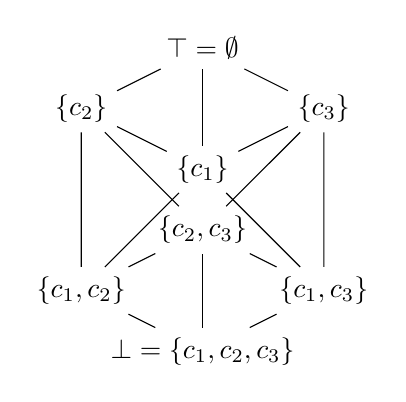
\begin{tikzpicture}[scale=0.77,auto]

% single PVS
\node (bot) at (0,0) {$\bot = \{c_1, c_2, c_3 \}$};
\node (c1c2) at (-2,1) {$\{c_1, c_2\}$};
\node (c2c3) at (0,2) {$\{c_2, c_3\}$};
\node (c1c3) at (2,1) {$\{c_1, c_3\}$};

\node (c1) at (0,3) {$\{c_1\}$};
\node (c2) at (-2,4) {$\{c_2\}$};
\node (c3) at (2,4) {$\{c_3\}$};
%\node (a) at (-1,0.5) {$a$};
%\node (b) at (-1,1.5) {$b$};
%\node (c) at (1,1) {$c$};
\node (top) at (0,5) {$\top = \emptyset$};


\path[-]
(bot) edge (c1c2)
      edge (c2c3)
      edge (c1c3)
(c1c2) edge (c2c3)
(c1c3) edge (c2c3)
(c1c3) edge (c1)
(c1c3) edge (c3)
(c2c3) edge (c2)
(c2c3) edge (c3)
(c1c2) edge (c1)
(c1c2) edge (c2)
(c1) edge (c2)
(c1) edge (c3)
(c2) edge (top)
(c1) edge (top)
(c3) edge (top)
      ;
%(a) edge (b)
%(b) edge (top)
%(bot) edge (c)
%(c) edge (top)
;

\end{tikzpicture}
\end{center}
\label{fig:nosuprema}
\end{figure}
%\onslide<0>{
\begin{lstlisting}
%
% Typical Optimization Routine (Branch and Bound):
%
%  1. Look for the first feasible solution
%  2. Impose restrictions on the next feasible solution
%  3. Repeat
\end{lstlisting}
%}
\begin{textblock*}{2.5cm}[1,1](\textwidth-8.5cm,\textheight-4.03cm)
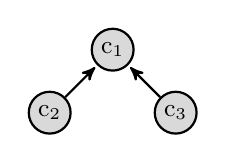
\begin{tikzpicture}[auto,
                    ->,>=stealth',shorten >=1pt,thick,
                    node distance=.7cm,inner sep=2pt,
                    constraint/.style={circle,fill=black!15,draw,font=\sffamily\small}]
\node[constraint node] (1) at (0, 0)                   {$\mathrm{c}_1$};
\node[constraint node] (2) at ($ (1) + (-0.8, -0.8) $) {$\mathrm{c}_2$};  
\node[constraint node] (3) at ($ (1) + ( 0.8, -0.8) $) {$\mathrm{c}_3$};  
%  
\path[every node/.style={font=\sffamily\tiny}]
  (2) edge (1)
  (3) edge (1)
  ;
\end{tikzpicture}
\end{textblock*}
\end{frame}


\tikzset{onslide/.code args={<#1>#2}{%
  \only<#1>{\pgfkeysalso{#2}}
}}
\tikzstyle{highlight}=[isseorange,ultra thick]
\tikzstyle{highlight2}=[CornflowerBlue,ultra thick]

\begin{frame}[fragile]{Search types: Strictly better}
The whole valuation space (partially ordered)



\begin{figure}[!t]
\begin{center}
\begin{tikzpicture}[scale=0.77,auto]

% single PVS
\node (bot) at (0,0) {\alert{$\bot = \{c_1, c_2, c_3 \}$}};
\node (c1c2) at (-2,1) {\alert<2->{$\{c_1, c_2\}$}};
\node (c2c3) at (0,2) {$\{c_2, c_3\}$};
\node (c1c3) at (2,1) {$\{c_1, c_3\}$};

\node (c1) at (0,3) {\alert<3->{$\{c_1\}$}};
\node (c2) at (-2,4) {\alert<4->{$\{c_2\}$}};
\node (c3) at (2,4) {$\{c_3\}$};
%\node (a) at (-1,0.5) {$a$};
%\node (b) at (-1,1.5) {$b$};
%\node (c) at (1,1) {$c$};
\node (top) at (0,5) {$\top = \emptyset$};


\path[-]
(bot) edge[onslide={<2->{highlight}}] (c1c2)
      edge (c2c3)
      edge (c1c3)
(c1c2) edge (c2c3)
(c1c3) edge (c2c3)
(c1c3) edge (c1)
(c1c3) edge (c3)
(c2c3) edge (c2)
(c2c3) edge (c3)
(c1c2) edge[onslide={<3->{highlight}}] (c1)
(c1c2) edge (c2)
(c1) edge[onslide={<4->{highlight}}] (c2)
(c1) edge (c3)
(c2) edge (top)
(c1) edge (top)
(c3) edge (top)
      ;
%(a) edge (b)
%(b) edge (top)
%(bot) edge (c)
%(c) edge (top)
;

\end{tikzpicture}
\end{center}
\label{fig:nosuprema}
\end{figure}
\begin{lstlisting}
function ann: strictlyBetterBAB(var set of SOFTCONSTRAINTS: vScs) 
      = repeat(
           if next() then 
             commit() /\ 
             post(isWorse(sol(vScs), vScs))
           else break endif       );
\end{lstlisting}
\begin{textblock*}{2.5cm}[1,1](\textwidth-8.5cm,\textheight-4.03cm)
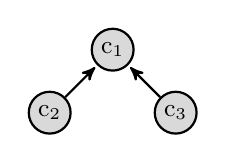
\begin{tikzpicture}[auto,
                    ->,>=stealth',shorten >=1pt,thick,
                    node distance=.7cm,inner sep=2pt,
                    constraint/.style={circle,fill=black!15,draw,font=\sffamily\small}]
\node[constraint node] (1) at (0, 0)                   {$\mathrm{c}_1$};
\node[constraint node] (2) at ($ (1) + (-0.8, -0.8) $) {$\mathrm{c}_2$};  
\node[constraint node] (3) at ($ (1) + ( 0.8, -0.8) $) {$\mathrm{c}_3$};  
%  
\path[every node/.style={font=\sffamily\tiny}]
  (2) edge (1)
  (3) edge (1)
  ;
\end{tikzpicture}
\end{textblock*}
\end{frame}

\begin{frame}[fragile]{Search types: Only not dominated}
The whole valuation space (partially ordered)

\begin{figure}[!t]
\begin{center}
\begin{tikzpicture}[scale=0.77,auto]

% single PVS
\node (bot) at (0,0) {\alert{$\bot = \{c_1, c_2, c_3 \}$}};
\node (c1c2) at (-2,1) {\alert<2->{$\{c_1, c_2\}$}};
\node[onslide={<4->{highlight2}}] (c2c3) at (0,2) {$\{c_2, c_3\}$};
\node (c1c3) at (2,1) {$\{c_1, c_3\}$};

\node (c1) at (0,3) {\alert<3->{$\{c_1\}$}};
\node (c2) at (-2,4) {\alert<5->{$\{c_2\}$}};
\node [onslide={<6->{highlight2}}](c3) at (2,4) {$\{c_3\}$};
%\node (a) at (-1,0.5) {$a$};
%\node (b) at (-1,1.5) {$b$};
%\node (c) at (1,1) {$c$};
\node (top) at (0,5) {$\top = \emptyset$};


\path[-]
(bot) edge[onslide={<2->{highlight}}] (c1c2)
      edge (c2c3)
      edge (c1c3)
(c1c2) edge[onslide={<4->{highlight2}}] (c2c3)
(c1c3) edge (c2c3)
(c1c3) edge (c1)
(c1c3) edge (c3)
(c2c3) edge (c2)
(c2c3) edge[onslide={<6->{highlight2}}] (c3)
(c1c2) edge[onslide={<3->{highlight}}] (c1)
(c1c2) edge (c2)
(c1) edge[onslide={<5->{highlight}}] (c2)
(c1) edge (c3)
(c2) edge (top)
(c1) edge (top)
(c3) edge (top)
      ;

\end{tikzpicture}
\end{center}
\label{fig:nosuprema}
\end{figure}
\begin{lstlisting}
function ann: onlyNotDominatedBAB(var set of SOFTCONSTRAINTS: vScs) 
      = repeat(
           if next() then 
             commit() /\ 
             post((isWorse(vScs, sol(vScs)) \/ vScs = sol(vScs)))
           else break endif       );
\end{lstlisting}
\begin{textblock*}{2.5cm}[1,1](\textwidth-8.5cm,\textheight-4.03cm)
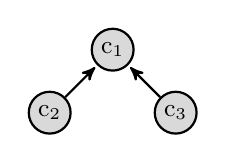
\begin{tikzpicture}[auto,
                    ->,>=stealth',shorten >=1pt,thick,
                    node distance=.7cm,inner sep=2pt,
                    constraint/.style={circle,fill=black!15,draw,font=\sffamily\small}]
\node[constraint node] (1) at (0, 0)                   {$\mathrm{c}_1$};
\node[constraint node] (2) at ($ (1) + (-0.8, -0.8) $) {$\mathrm{c}_2$};  
\node[constraint node] (3) at ($ (1) + ( 0.8, -0.8) $) {$\mathrm{c}_3$};  
%  
\path[every node/.style={font=\sffamily\tiny}]
  (2) edge (1)
  (3) edge (1)
  ;
\end{tikzpicture}
\end{textblock*}
\end{frame}

\begin{frame}[fragile]{Search Demo: Model}
\lstinputlisting{models/diff-BAB.mzn}
\end{frame}

\begin{frame}[fragile]{Search Demo: Strictly better}
Execute \texttt{minisearch diff-BAB-sb.mzn } 

(explores in order $\{c_3\}, \{c_2\}, \{c_1\}$)



\begin{figure}[!t]
\begin{center}
\begin{tikzpicture}[scale=0.7,auto]

% single PVS
\node (bot) at (0,0) {\alert{$\bot = \{c_1, c_2, c_3 \}$}};
\node (c1c2) at (-2,1) {$\{c_1, c_2\}$};
\node (c2c3) at (0,2) {$\{c_2, c_3\}$};
\node (c1c3) at (2,1) {$\{c_1, c_3\}$};

\node (c1) at (0,3) {$\{c_1\}$};
\node (c2) at (-2,4) {$\{c_2\}$};
\node (c3) at (2,4) {\alert<2->{$\{c_3\}$}};
%\node (a) at (-1,0.5) {$a$};
%\node (b) at (-1,1.5) {$b$};
%\node (c) at (1,1) {$c$};
\node (top) at (0,5) {$\top = \emptyset$};


\path[-]
(bot) edge (c1c2)
      edge (c2c3)
      edge (c1c3)
      edge (c2)
      edge[onslide={<2->{highlight}}] (c3)
(c1c2) edge (c2c3)
(c1c3) edge (c2c3)
(c1c3) edge (c1)
(c1c3) edge (c3)
(c2c3) edge (c2)
(c2c3) edge (c3)
(c1c2) edge (c1)
(c1c2) edge (c2)
(c1) edge (c2)
(c1) edge (c3)
(c2) edge (top)
(c1) edge (top)
(c3) edge (top)
      ;
%(a) edge (b)
%(b) edge (top)
%(bot) edge (c)
%(c) edge (top)
;

\end{tikzpicture}
\end{center}
\label{fig:nosuprema}
\end{figure}
\small
\begin{lstlisting}
% just sees {c_3} then finds no better solution and stops
% 
Intermediate solution: Obj: 1 violating {3..3}: x=3
----------
==========
%
\end{lstlisting}

\begin{textblock*}{2.5cm}[1,1](\textwidth-8.5cm,\textheight-4.03cm)
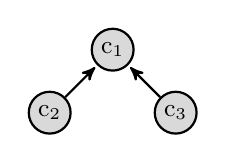
\begin{tikzpicture}[auto,
                    ->,>=stealth',shorten >=1pt,thick,
                    node distance=.7cm,inner sep=2pt,
                    constraint/.style={circle,fill=black!15,draw,font=\sffamily\small}]
\node[constraint node] (1) at (0, 0)                   {$\mathrm{c}_1$};
\node[constraint node] (2) at ($ (1) + (-0.8, -0.8) $) {$\mathrm{c}_2$};  
\node[constraint node] (3) at ($ (1) + ( 0.8, -0.8) $) {$\mathrm{c}_3$};  
%  
\path[every node/.style={font=\sffamily\tiny}]
  (2) edge (1)
  (3) edge (1)
  ;
\end{tikzpicture}
\end{textblock*}
\end{frame}


\begin{frame}[fragile]{Search Demo: Only not dominated}
Execute \texttt{minisearch diff-BAB-ond.mzn}

(explores in order $\{c_3\}, \{c_2\}, \{c_1\}$)

\begin{figure}[!t]
\begin{center}
\begin{tikzpicture}[scale=0.7,auto]

% single PVS
\node (bot) at (0,0) {\alert{$\bot = \{c_1, c_2, c_3 \}$}};
\node (c1c2) at (-2,1) {$\{c_1, c_2\}$};
\node (c2c3) at (0,2) {$\{c_2, c_3\}$};
\node (c1c3) at (2,1) {$\{c_1, c_3\}$};

\node (c1) at (0,3) {$\{c_1\}$};
\node [onslide={<3->{highlight2}}] (c2) at (-2,4) {$\{c_2\}$};
\node [onslide={<2->{highlight}}] (c3) at (2,4) {$\{c_3\}$};
%\node (a) at (-1,0.5) {$a$};
%\node (b) at (-1,1.5) {$b$};
%\node (c) at (1,1) {$c$};
\node (top) at (0,5) {$\top = \emptyset$};


\path[-]
(bot) edge (c1c2)
      edge (c2c3)
      edge (c1c3)
      edge[onslide={<2->{highlight}}] (c3)
      edge[onslide={<3->{highlight2}}] (c2)
(c1c2) edge (c2c3)
(c1c3) edge (c2c3)
(c1c3) edge (c1)
(c1c3) edge (c3)
(c2c3) edge (c2)
(c2c3) edge (c3)
(c1c2) edge (c1)
(c1c2) edge (c2)
(c1) edge (c2)
(c1) edge (c3)
(c2) edge (top)
(c1) edge (top)
(c3) edge (top)
      ;

\end{tikzpicture}
\end{center}
\label{fig:nosuprema}
\end{figure}
\begin{lstlisting}
% lists both solutions
Intermediate solution: Obj: 1 violating {3..3}: x=3
----------
Intermediate solution: Obj: 1 violating {2..2}: x=2
----------
==========
\end{lstlisting}
\begin{textblock*}{2.5cm}[1,1](\textwidth-8.5cm,\textheight-4.03cm)
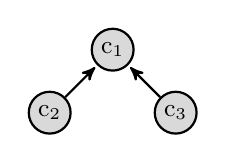
\begin{tikzpicture}[auto,
                    ->,>=stealth',shorten >=1pt,thick,
                    node distance=.7cm,inner sep=2pt,
                    constraint/.style={circle,fill=black!15,draw,font=\sffamily\small}]
\node[constraint node] (1) at (0, 0)                   {$\mathrm{c}_1$};
\node[constraint node] (2) at ($ (1) + (-0.8, -0.8) $) {$\mathrm{c}_2$};  
\node[constraint node] (3) at ($ (1) + ( 0.8, -0.8) $) {$\mathrm{c}_3$};  
%  
\path[every node/.style={font=\sffamily\tiny}]
  (2) edge (1)
  (3) edge (1)
  ;
\end{tikzpicture}
\end{textblock*}
\end{frame}


\begin{frame}[fragile]{Switching PVS Type}
Concrete PVS are instantiated by importing the appropriate \texttt{pvs\_x.mzn} file.
\lstinputlisting{models/m1.mzn}
\end{frame}

\begin{frame}[fragile]{Consistency Checks}
Vital, when designing constraint relationships: \alert{avoid cycles!}

\texttt{model-inconsistent.mzn}
\lstinputlisting{models/model-inconsistent.mzn}
\end{frame}

\begin{frame}[fragile]{Consistency Checks}
\begin{center}
\includegraphics[width=.7\textwidth]{img/errorMz.png}
\end{center}
Better: Add model checks to detect cyclic relationships!
\end{frame}

\begin{frame}[fragile]{Consistency Checks: Assertions}
\texttt{model-inconsistent-safe.mzn}
\lstinputlisting{models/model-inconsistent-safe.mzn}
\end{frame}

\begin{frame}[fragile]{Consistency Checks: Assertions}
\texttt{minisearch model-inconsistent-safe.mzn}

\vspace*{2ex}

\begin{verbatim}
minizinc/std/soft_constraints/cr_consistency.mzn:46:
  in call 'assert'
  Assertion failed: Relationship is cyclic!

\end{verbatim}

\end{frame}

\begin{frame}[fragile]{Transitive Closure}
\vspace*{2ex}

For larger constraint relationships, it can be more convenient 
to just specify a directed acyclic graph and have the closure (all transitive edges)
be calculated automatically.

\centering
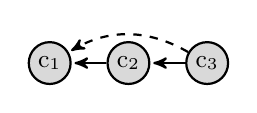
\begin{tikzpicture}[auto,
                    ->,>=stealth',shorten >=1pt,thick,
                    node distance=.7cm,inner sep=2pt,
                    constraint/.style={circle,fill=black!15,draw,font=\sffamily\small}]
\node[constraint node] (1) at (0, 0)                   {$\mathrm{c}_1$};
\node[constraint node] (2) at ($ (1) + (1, 0) $) {$\mathrm{c}_2$};  
\node[constraint node] (3) at ($ (1) + ( 2, 0) $) {$\mathrm{c}_3$};  
%  
\path[every node/.style={font=\sffamily\tiny}]
  (2) edge (1)
  (3) edge (2)
  (3) edge[dashed,bend right] (1)
  ;
\end{tikzpicture}
\lstinputlisting{models/cr_trans_example.mzn}
\end{frame}

\begin{frame}[fragile]{Variable Ordering}
Recall that \texttt{soft\_constraints.mzn} defines a variable ordering with 
weights in descending order:

\vspace*{1ex}

\begin{lstlisting}
% find the sorted permutation of soft constraint instances
array[SOFTCONSTRAINTS] of SOFTCONSTRAINTS: sortPermScs = 
    arg_sort(penalties);
% invert, since arg_sort use <= and we need decreasing order
array[SOFTCONSTRAINTS] of SOFTCONSTRAINTS: mostImpFirst = 
    [ sortPermScs[nScs-s+1] | s in SOFTCONSTRAINTS]; 

\end{lstlisting}

\vspace*{1ex}

We can use this ordering to try out important constraints early on in search.
\end{frame}

\begin{frame}[fragile]{Variable Ordering: Demo}
\texttt{smallexample.mzn}:

\lstinputlisting{models/smallexample.mzn}
\small 
\begin{verbatim}
Obj: 4 by x=1, y=1,z=1
----------
Obj: 3 by x=1, y=1,z=3
----------
Obj: 1 by x=1, y=2,z=1
----------
==========
\end{verbatim}
\end{frame}

\begin{frame}[fragile]{Variable Ordering: Demo}
\texttt{smallexample-mif.mzn}:

\lstinputlisting{models/smallexample-mif.mzn}
\small 
\begin{verbatim}
Obj: 1 by x=1, y=2,z=1
----------
==========
\end{verbatim}
(finds the optimal solution at first try)
\end{frame}

\begin{frame}[fragile]{Variable Ordering: Demo}
This ordering can of course be combined with problem-specific heuristics 
(e.g. large rectangles first in packing problems, here first-fail on a queens problem).

\vspace*{2ex}
Example: \texttt{minisearch soft-queens.mzn}
\begin{lstlisting}
solve :: seq_search([
         int_search([satisfied[mostImpFirst[i]] | i in SOFTCONSTRAINTS], 
                     input_order, indomain_max, complete),
         int_search(
           queens, 
           first_fail,
           indomain_median,
           complete
       )] ) 
     minimize penSum;
\end{lstlisting}
\end{frame}



\begin{frame}[fragile]{Redundant Constraints}
If we are mostly interested in performance (for constraint-relationship-based search), 
we can add \emph{redundant constraints}, if we use \emph{strictlyBetter} search.

\vspace*{2ex}

From \texttt{redundant-constraints.mzn}:
\begin{lstlisting}
constraint spd_worse({1}, violatedScs,SOFTCONSTRAINTS,crEdges);
% if we need to find an actually better solution than {1}
% (with violation 2), the penalty sum has to be strictly
% less than 2
constraint penSum < 2;
\end{lstlisting}
\end{frame}

\begin{frame}{Redundant Constraints}

\begin{center}
Without redundant constraint (\texttt{redundant-constraints.mzn}):

\includegraphics[width=.6\textwidth]{img/withoutred.png}

\vspace*{3ex}

With redundant weight constraint -- less failures (\texttt{redundant-constraints-weighted.mzn}):

\includegraphics[width=.4\textwidth]{img/withred.png}
\end{center}
\end{frame}

\begin{frame}[fragile]{Custom Search}
Search strategies based on PVS are defined in \texttt{soft\_constraints/pvs\_search.mzn}.

\vspace*{2ex}

Currently supported:
\begin{itemize}
\item Branch and bound (BAB)
\item Large Neighborhood Search (LNS)
\end{itemize}

\vspace*{2ex}

for \emph{strictly better} and \emph{only not dominated}

\begin{lstlisting}
%[... in m2.mzn]
solve
search strictlyBetterBAB(violatedScs) /\ print();

%[... in m2-lns.mzn]
solve 
search lns_pvs(violatedScs, dummies, 2, 0.5) /\ print();
\end{lstlisting}

\end{frame}

\begin{frame}{Summary}
This concludes our overview of some language features


\vspace*{2ex}

Make sure to check out our other slides about:
\begin{itemize}
\item Step-by-Step enhancing a MiniZinc model (establishes the core elements)
\item Case Studies (for some specific examples)
\end{itemize}

\vspace*{2ex}

\url{http://isse-augsburg.github.io/constraint-relationships/}
\end{frame}

\begin{frame}[allowframebreaks]
        \frametitle{References}
        \bibliographystyle{apalike}
        \bibliography{references.bib,../common.bib}
\end{frame}


\end{document}

